\documentclass[12pt]{article}

%\usepackage{scicite}

%\usepackage{times}
\usepackage{pdfpages}

%\usepackage[ansinew]{inputenc}
\usepackage{amsmath}
\usepackage{siunitx}
\usepackage[colorlinks=true, urlcolor=blue, linkcolor=blue,citecolor=blue]{hyperref}
%\usepackage[german]{babel}
\usepackage{float}
%\usepackage[numbers]{natbib}
\usepackage[authoryear]{natbib}
%\usepackage[pliannatuthoryear]{natbib}

\usepackage{graphicx}
\graphicspath{{/home/mpim/m300524/MSc_Thesis/gfx/}}

% The following parameters seem to provide a reasonable page setup.

\topmargin 0.0cm
\oddsidemargin 0.2cm
\textwidth 16cm 
\textheight 21cm
\footskip 1.0cm

%\newcommand{\member}{m105_1994_2001}
%\newcommand{\member}{m178_1985_1992} % zweitbesten
\newcommand{\member}{m182_1988_1995} %funktioniert am besten

%The next command sets up an environment for the abstract to your paper.

%\newenvironment{sciabstract}{%
%\begin{quote} \bf}
%{\end{quote}}


% If your reference list includes text notes as well as references,
% include the following line; otherwise, comment it out.

\renewcommand\refname{References and Notes}

% The following lines set up an environment for the last note in the
% reference list, which commonly includes acknowledgments of funding,
% help, etc.  It's intended for users of BibTeX or the {thebibliography}
% environment.  Users who are hand-coding their references at the end
% using a list environment such as {enumerate} can simply add another
% item at the end, and it will be numbered automatically.

%\newcounter{lastnote}
%\newenvironment{scilastnote}{%
%\setcounter{lastnote}{\value{enumiv}}%
%\addtocounter{lastnote}{+1}%
%\begin{list}%
%{\arabic{lastnote}.}
%{\setlength{\leftmargin}{.22in}}
%{\setlength{\labelsep}{.5em}}}
%{\end{list}}


% Include your paper's title here

\title{The impact of biology on decadal decreasing trends of carbon sink in the Southern Ocean} 


\author
{Aaron Spring,$^{1\ast}$ Hongmei Li,$^{1}$ Tatiana Ilyina$^{1}$\\
\\
\normalsize{$^{1}$Max Planck Institute for Meteorology, Bundesstra{\ss}e 53, 20146 Hamburg, Germany}\\
\\
\normalsize{$^\ast$To whom correspondence should be addressed; E-mail:  aaron.spring@mpimet.mpg.de.}
}

% Include the date command, but leave its argument blank.

\date{}



%%%%%%%%%%%%%%%%% END OF PREAMBLE %%%%%%%%%%%%%%%%




\begin{document} 

% Double-space the manuscript.

\baselineskip24pt

% Make the title.

\maketitle 
%Other title: The response of biology for the Southern Ocean carbon sink under the context of intensified winds

\vspace{3cm}
\textbf{Key points:}

\begin{itemize}
\item Large ensebmle simulations are able to reproduce decadal decreasing trends in the Southern Ocean carbon sink
\item Internal variability of the Southern Ocean carbon uptake links to primary production
\item Southern Ocean carbon sink is sensitive to stability of the water column which is needed for primary production blooms
\end{itemize}



% Place your abstract within the special {sciabstract} environment.
\newpage

\begin{abstract}
\baselineskip24pt
  The Southern Ocean is a major sink for anthropogenic CO$_2$ emissions and hence it plays an essential role in modulating global carbon cycle and climate change. Previous studies based on observations show pronounced decadal variations of carbon uptake in the Southern Ocean in recent decades and this variability is largely driven by internal climate variability. However, due to limited ensemble size of simulations, the variability of this important ocean sink is still poorly assessed by the state-of-the-art earth system models (ESMs). To assess the internal variability of carbon sink in the Southern Ocean, we use a large ensemble of 100 member simulations based on the Max Planck Institute-ESM (MPI-ESM). Here we use model simulations from 1980-2015 to compare with available observation-based dataset. We found several ensemble members showing decadal decreasing trends in the carbon sink, which are similar to the trend shown in observations. This result suggests that MPI-ESM large ensemble simulations are able to reproduce decadal variation of carbon sink in the Southern Ocean. Moreover, the decreasing trends of Southern Ocean carbon sink in MPI-ESM are mainly contributed by region between 50-60$^\circ$S. %To understand the internal variability of the air-sea carbon fluxes in the Southern Ocean, we further investigate the variability of underlying processes, such as physical climate variability and ocean biological processes. 
Our results focus on the impact of biology on decadal decreasing trends of carbon sink. Primary production is reduced in area from 50-60$^\circ$S due to a reduced euphotic water column stability; therefore the biological drawdown of ocean surface pCO$_2$ is weakened accordingly and hence the Southern Ocean carbon sink is decreasing.
  
\end{abstract}



% In setting up this template for *Science* papers, we've used both
% the \section* command and the \paragraph* command for topical
% divisions.  Which you use will of course depend on the type of paper
% you're writing.  Review Articles tend to have displayed headings, for
% which \section* is more appropriate; Research Articles, when they have
% formal topical divisions at all, tend to signal them with bold text
% that runs into the paragraph, for which \paragraph* is the right
% choice.  Either way, use the asterisk (*) modifier, as shown, to
% suppress numbering.

\newpage

\section{Introduction}


The oceans are major carbon sink by taking up about 25-30\% of the anthropogenic carbon emissions from the atmosphere \citep{Quere2016}. As a major sink, the Southern Ocean contributes about 40\% to the global ocean carbon sink \citep{Sabine2004}. The Southern Ocean carbon sink shows large variability on decadal time-scale \citep{landschuetzer2015}. However, the processes responsible for the decadal variations of the Southern Ocean carbon sink is still not clear.

%The oceans are major carbon sink by taking up about 25-30\% of the anthropogenic carbon emissions from the atmosphere \citep{Quere2016}. The Southern Ocean connects all major ocean basins and therefore has an important role for the global water mass distribution. It is also a large contributor of 40\% for the global anthropogenic oceanic carbon sink \citep{Sabine2004}.

The evolution of the Southern Ocean carbon sink shows large variability \citep{landschuetzer2015}. Moreover, observation-based estimates suggest the  Southern Ocean carbon sink weakened in the 1990s despite the increase of atmospheric pCO$_2$ forcing and reinvigorated in the beginning of the 21$^{st}$ century \citep{LeQuere2007,landschuetzer2015}. Due to sparse and fairly recent observational samples and diverse mapping methods, observation-based estimates of the Southern Ocean carbon sink have a large spread, which limits the investigation of possible mechanisms in regulating the variations of the oceanic carbon sink in the Southern Ocean.  \citep{LeQuere2007,Roedenbeck2013,landschuetzer2015}. 


%The evolution of the Southern Ocean carbon sink shows large variability \citep{landschuetzer2015}. However, observation-based estimates suggest a weakening of the Southern Ocean carbon sink in the 1990s against the forced signal of atmospheric pCO$_2$ increase \citep{landschuetzer2015,LeQuere2007}. Due to sparse and fairly recent observational samples and diverse mechanism of calculation, observation-based estimates of the Southern Ocean carbon sink have a large spread \citep{LeQuere2007,Roedenbeck2013,landschuetzer2015}. 

The decreasing trend of Southern Ocean carbon sink in the 1990s is explained by intensified westerly winds which lead to enhanced upwelling of carbon-rich waters \citep{LeQuere2007}. This causality was also confirmed by forced model results associated with positive states in the Southern Annular Mode (SAM) indicating intensified winds \citep{Lovenduski2007}. The influence of SAM on the carbon sink on decadal timescales has been demonstrated in an ocean-only simulation forced with historical data from National Centers for Environmental Prediction (NCEP) \citep{Lovenduski2008}. In all those studies, biology was found to be not changing significantly, and thus not included in an explanation for a decadal trend. As shown in Landsch{\"u}tzer et al. (2015), the carbon sink in the Southern Ocean reinvigorated, although the Southern Ocean westerlies, which are closely linked to SAM, continued to increase. It suggests that the SAM may not be the only driver of the ocean carbon sink changes in the Southern Ocean, and other processes, such as biology, may play an important role in regulating the carbon fluxes.   


However, model studies suggest that changes in circulation also affect the biological pump in the Southern Ocean \citep{Sarmiento1998}. As deduced from satellite observations from 1997-2004 and forced models on different timescales, intensified winds in the context of increasing SAM change the Southern Ocean circulation and enhance nutrient supply, and hence increase the biological production \citep{Lovenduski2005,Hauck2013,wang2012}. The role of biology on decadal trends in a freely coupled model remains unadressed.

Model simulations are a useful complementary method to study variations, their driving processes and the consequences for biogeochemical cycles. Multi-model intercomparison exercises, such as Coupled Model Intercomparison Project Phase 5 (CMIP5) indicate that evolution of the Southern Ocean carbon uptake is quite robustly projected to increase in the models \citep{Wang2016}. 
%Internal variability, like anomalous decadal trends, can be studied in large ensemble simulations, such as the separation of trends from internal variability in the ocean carbon sink \citep{McKinley2016}. 
Large ensemble simulations of a single model isolate the model uncertainty and enable us to investigate internal variability \citep{McKinley2016}. Observation could be one realization from a large ensemble simulations. Therefore, it is possible to find some ensemble members which show an evolution of the Southern Ocean carbon sink similar to observations, and we could further use the model output to help us understand the underlying mechanisms.

By using a large ensemble simulation based on the Max-Planck-Institute Earth System Model (MPI-ESM), we investigate the variability of the oceanic carbon uptake. We try to answer the following questions: How large is the internal variability of the Southern Ocean carbon sink? Are large ensembles able to reproduce decreasing decadal trends of the Southern Ocean carbon sink? How does variability in physical processes influence biology and hence the carbon sink?

%outline


\section{Methods}

\subsection{Model description}
The MPI-ESM version 1.1 with a low-resolution configuration (MPI-ESM-LR) is used for the large ensemble simulations \citep{Giorgetta2013}. The atmosphere component ECHAM6.3 is on a T63 grid, corresponding to 1.9$^\circ$ at the equator (better would be values of high latitudes), with 47 vertical layers up to 0.01 hPa \citep{Stevens2013}. The ocean component MPI Ocean Model (MPIOM) has a horizontal resolution of 1.5$^\circ$ on average and 40 vertical levels \citep{Jungclaus2013}. The Hamburg Ocean Carbon Cycle Model (HAMOCC) \citep{Ilyina2013} represents the ocean biogeochemistry component of MPI-ESM. 
Atmospheric pCO$_2$ uses prescribed and well mixed values. The carbon cycle is not coupled (so called diagnostic), so effects of changes in the terrestrial or oceanic carbon sink are not reflected in pCO$_{2,atm}$ and hence terrestrial and oceanic carbon sink can not interact.

% about ensemble   
An ensemble of 100-member CMIP5 historical simulations and runs under  Representative Concentration Pathway (RCP) 4.5 scenario are integrated for the periods from 1850-2005, and 2006-2100, respectively. Ensemble members differ through starting from different year of the pre-industrial control simulation, so ocean and atmosphere have different initial conditions in each run.  
%ref to CESM ensemble or other ensemble studies?

\subsection{Data}
For comparison of CO$_2$flux with model simulations, we use the SOM-FFN data \citep{landschuetzer2015}.


\section{Results I: Historical evolution of the Southern Ocean carbon sink}

We focus our analysis on the recent three decades (eg. 1980-2015) when more ocean surface observation are available. On multi-decadal timescales, the carbon sink south of 35$^\circ$ south of the MPI-ESM 100-member simulations as well as SOM-FFN data increases and follows the atmospheric increase of pCO$_2$ (Fig. \ref{fig:evolution_southern_ocean_carbon_sink}). However, observations follow a decreasing carbon sink trend in the 1990s. The model simulation spreads in the Southern Ocean are of comparable magnitude as the uncertainty of SOM-FFN data. Previous studies assume gaussian statistics for large ensemble simulations \citep{Thompson2015}. We found the annular Southern Ocean carbon sink follows a normal distribution (Fig. SI \ref{fig:SOCS_temporal_gaussian} ). The large ensemble median represents the forced signal and the standard deviation represents internal variability \citep{Deser2012}. Internal variability, defined as the 1$\sigma$-spread of the 100-members, is constant over this period (~0.15$\pm$ 0.03 PgC yr$^{-1}$). SOM-FFN data ranges within the 2$\sigma$ ensemble spread. 

\begin{figure}
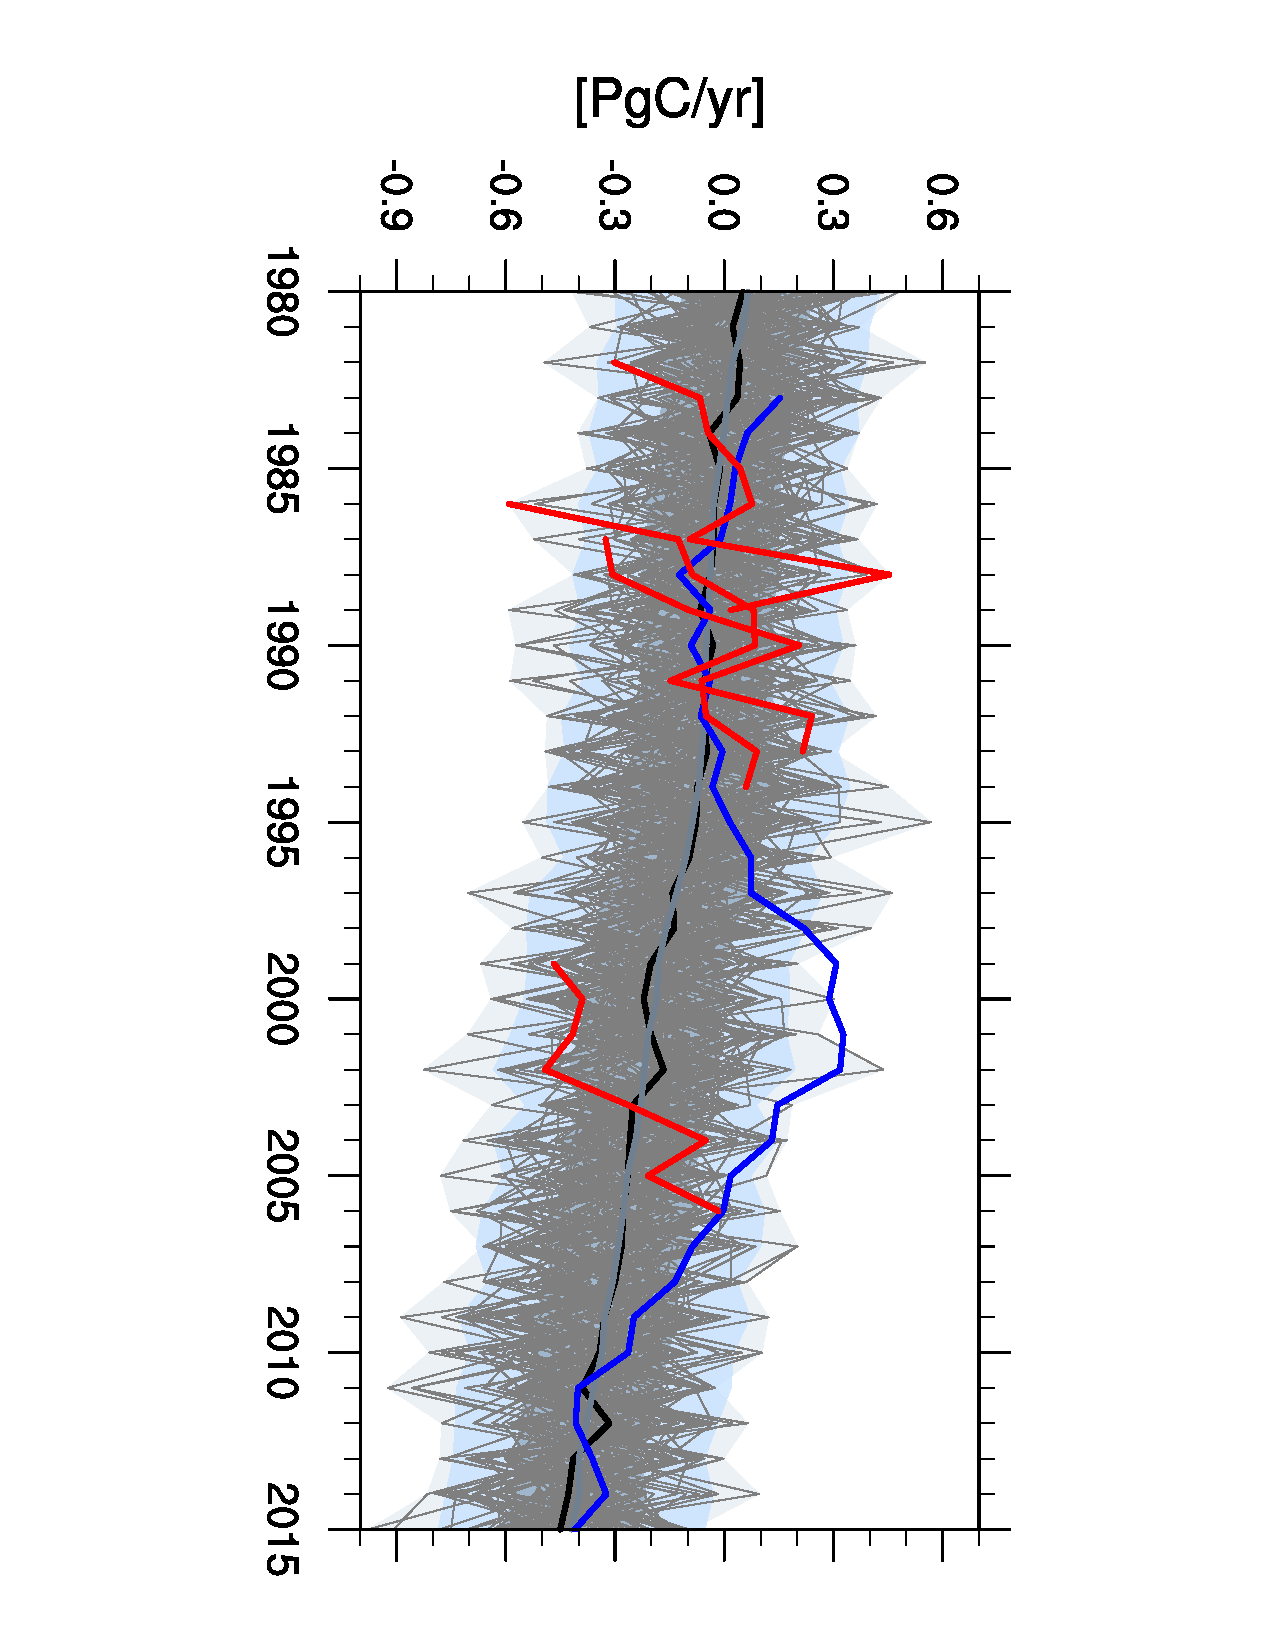
\includegraphics[scale=.55,angle=90,trim=4cm 0cm 4cm 0cm,clip]{co2flux_SO_timeseries_ym_mar-feb_35S_1980_2015_trend_8.pdf}
\caption{Evolution of the Southern Ocean carbon sink anomaly south of 35$^\circ$S. Grey lines show the 100 ensemble members, the black line the ensemble median, the gray shading is the range of the ensemble, the blue shading is the 2$\sigma$ ensemble spread, the red lines are decreasing sink trend candidates, the blue line is the SOM-FFN observation-based estimate; negative values indicate anomalous uptake with respect to the 1980s}
\label{fig:evolution_southern_ocean_carbon_sink}
\end{figure}

As an entry point of our analysis, we scan the dataset for trends similar to the anomalous outgassing trends of SOM-FFN data from the 1990s. To get a large sample size, we take running interval boundaries over the whole observational record of 1980-2015. Because of the strong seasonality in the high latitudes, we compute trends of the annual Southern Ocean carbon sink trend. The distribution of trends and the corresponding significance vary depending on the choosen length of trends (Fig. SI \ref{fig:heatmap}). A greatly monotonous trend of ten years only rarely occurs in 2600? available intervals. Most continuous trends only sustain for shorter than a decade. To ensure a certain number of monotonous trends and still a similar trendlength to a decade, we take 8-year trends in this analysis. For a meaningful analysis of the impact of biology, we separate the years between June and May, to ensure that a complete primary production bloom is captured in each year. Furthermore, the members used in this study are required to be monotonous similar to SOM-FFN data in the 1990s.
 
Applying those requirements, we find someamounttobechanged ensemble members with a decreasing decadal trend. They appear mostly in the first decades, because of increasing atmospheric pCO$_2$ forcing strengthens in later decades. These trend members are mostly in the 2$\sigma$ ensemble spread. 

%\newpage

\section{Results II: Spatial distribution of Southern Ocean carbon sink trend}

To get a deeper understand of the involved processes, we analyze spatial pattern of CO$_2$flux in the Southern Ocean. First, we see zonal structures in variables related to the carbon sink. To evaluate interval variability of the annual carbon sink, we analyze the CO$_2$flux distributions for each year in the 1990s from the whole ensemble.
The large ensemble median represents the forced signal and the standard deviation represents internal variability \citep{Deser2012}. The forced signal shows a dominant increasing trend in the Southern Ocean carbon sink (Fig. \ref{fig:SOCS_ensmean_ensstd} top left). Also in spatial distribution, the carbon sink in each grid point follows a normal distribution (Fig. SI \ref{fig:SOCS_temporal_gaussian}). The standard deviation (Fig. \ref{fig:SOCS_ensmean_ensstd} top right) shows differences in magnitude of internal variability in a zonal pattern. The largest internal variability appears in 50-60$^\circ$S south of the polar front. Internal variability drops north of 45$^\circ$S, showing the large internal variability of the Southern Ocean compared to other ocean basins.

Primary production also follows a zonal pattern (\ref{fig:SOCS_ensmean_ensstd} bottom left). Strongest plankton blooms occur around 40-55$^\circ$S. More light availability in lower latitudes enhances primary production whereas lower nutrient availability limits plankton growth further northwards.  Interestingly, the locations of large internal variability of in CO$_2$flux and primary production coincide.

\begin{figure}[h]
\centering
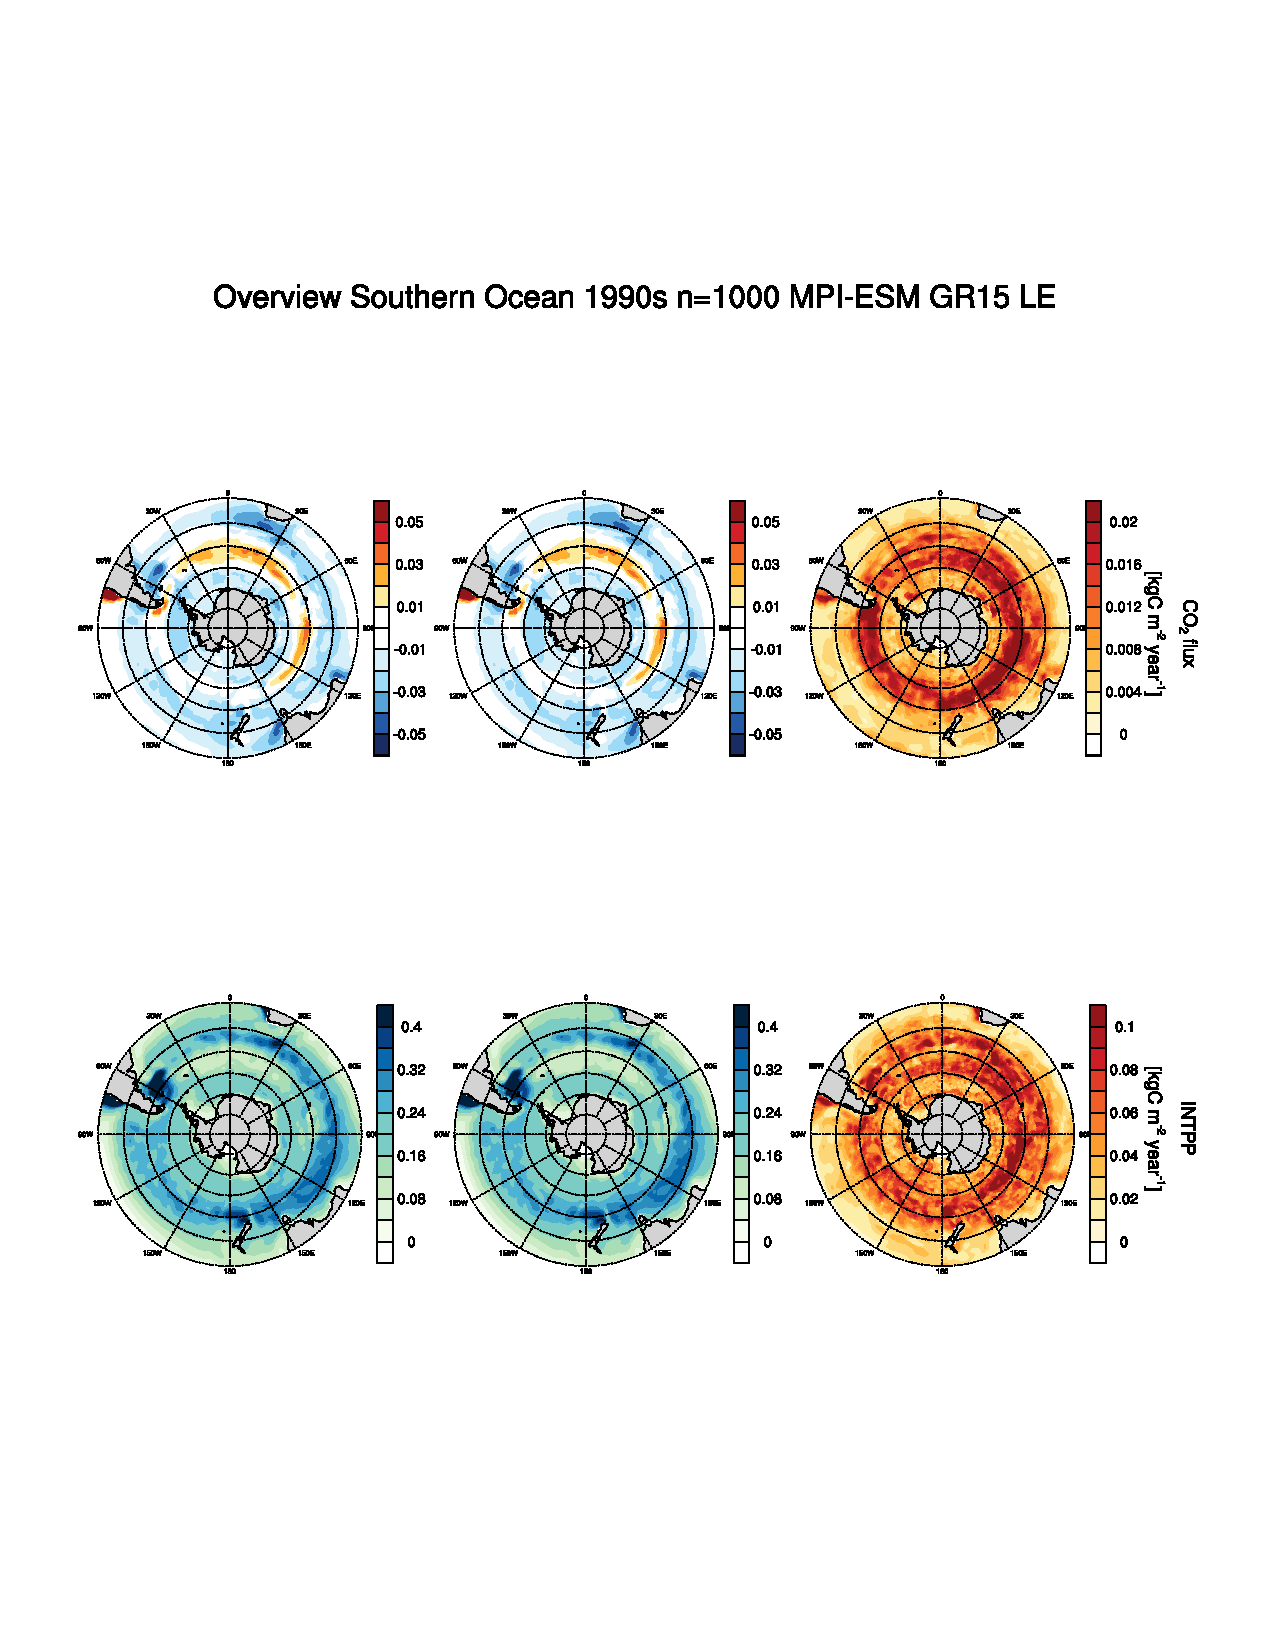
\includegraphics[scale=1.1,trim=7.2cm 15cm 0cm 8cm,clip]{Overview_SO_co2flux_intpp_ens_t1990s.pdf} % from gfx folder
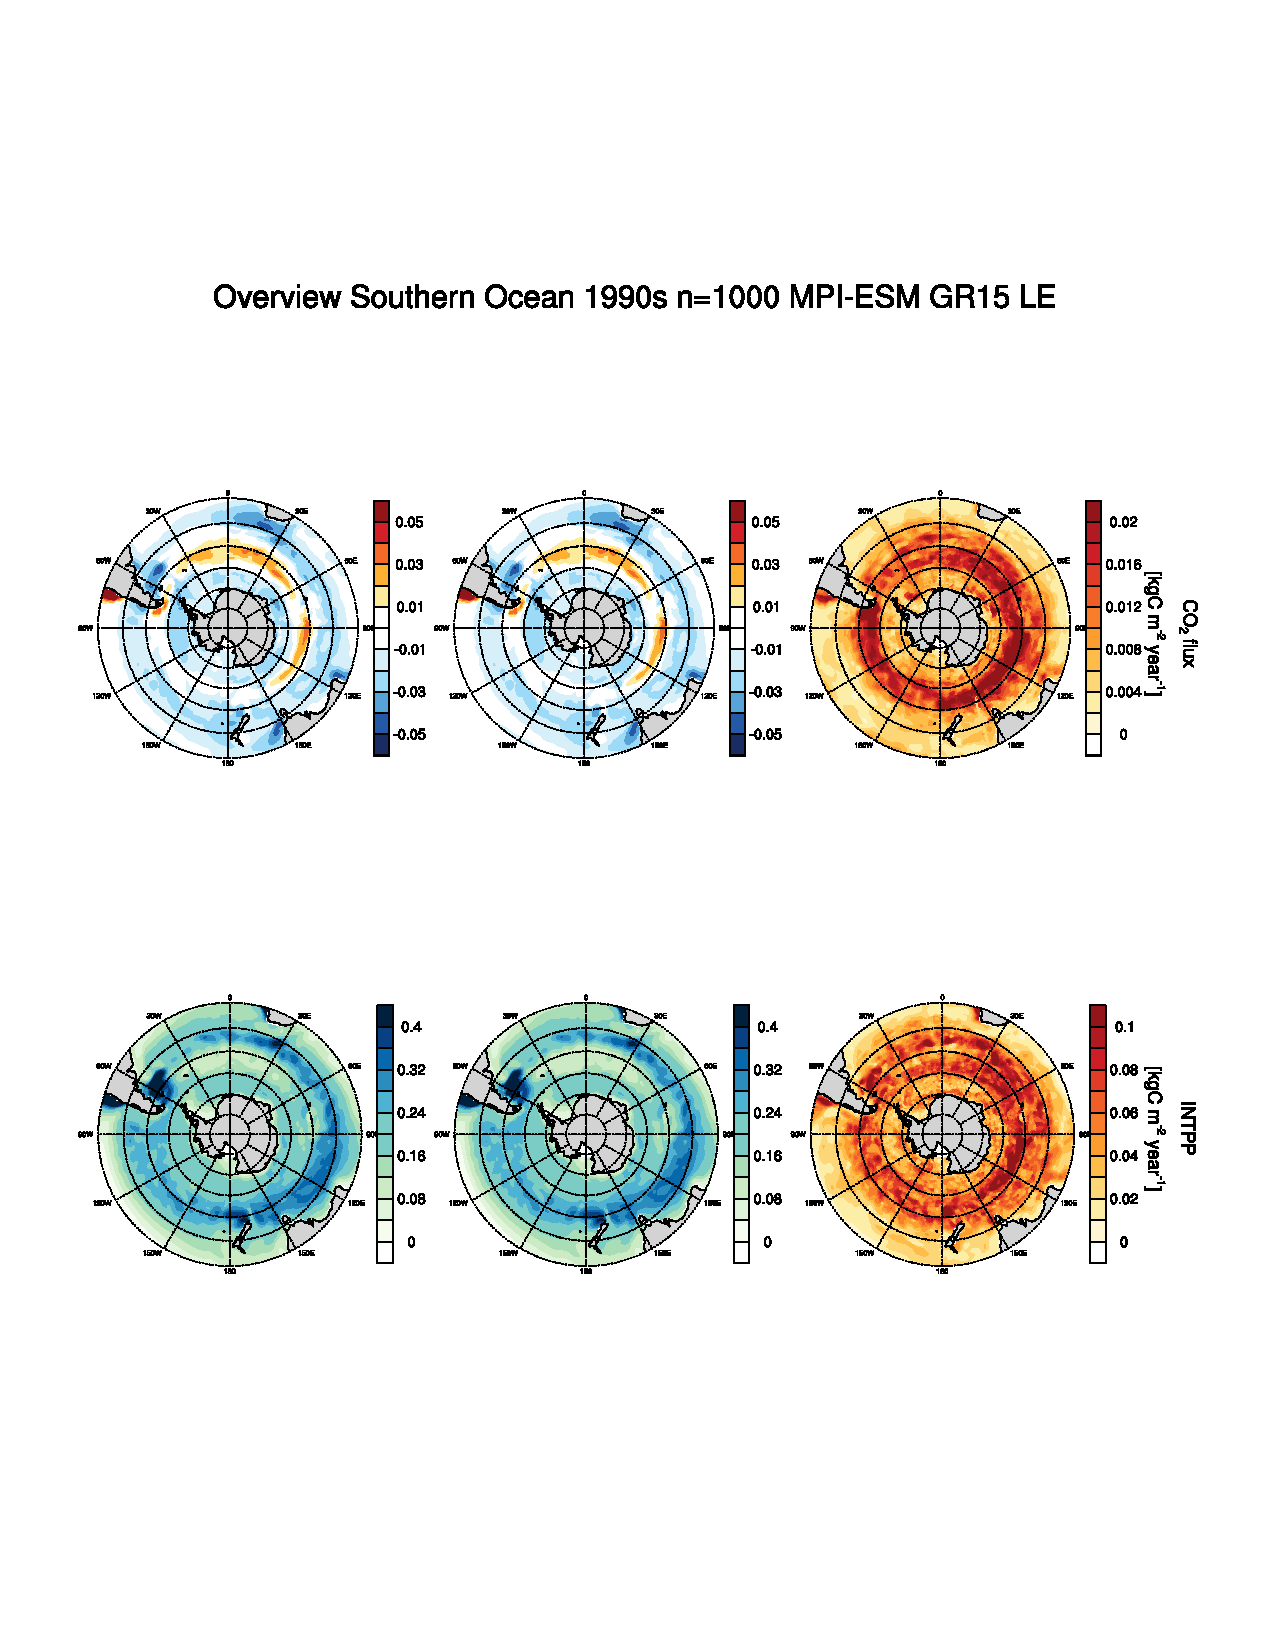
\includegraphics[scale=1.1,trim=7.2cm 6.3cm 0cm 16cm,clip]{Overview_SO_co2flux_intpp_ens_t1990s.pdf} % from gfx folder
\caption{Southern Ocean CO$_2$flux where negative values indicate ocean uptake (top) and primary production (bottom): ensemble median (left) as forced signal and ensemble standard deviation (right) as internal variability}
\label{fig:SOCS_ensmean_ensstd}
\end{figure}

Exemplary for all decadal decreasing carbon sink trend ensemble members, we show the most extreme case of anomalous outgassing. The underlying mechanism for decreasing carbon sink trends in our ensemble simulation seem to be of the same origin. The region of 50-60$^\circ$S has the strongest decreasing trend in CO$_2$flux.

As shown in previous studies \citep{LeQuere2007}, the variations of oceanic carbon uptake are related to the background thermal and dynamic changes. Insight to the drivers is gained by separating the pCO$_2$ seasonal amplitude in the thermal component driven by changes in sea surface temperature (Fig. SI \ref{fig:dpco2_separation}) and the non-thermal component driven by changes in DIC and/or alkalinity (Fig. SI \ref{fig:dpco2_separation}) \citep{Takahashi2002}. The non-thermal trend dominates the seasonal amplitude and decreases drastically in 50-60$^\circ$S, indicating that just the solubility change due to temperature is not the main driver.

Primary production and CO$_2$flux show opposing trend patterns as plankton growth takes up large amounts of surface DIC and hence lowers pCO$_2$ (Fig. \ref{fig:co2flux_intpp}). 
Temperature, nutrients and light availability can directly effect the phytoplankton growth rate. There are no significant trends in limiting factors found in the surface layers south of 40$^\circ$S. The Southern Ocean as an upwelling area has plenty of supply of nutrients from the deep ocean. Even in the austral summer months, the nutrient limitation factor for the average phytoplankton growth rate stays close to 1, which does not change the growth rate. (Fig. SI \ref{fig:nutrient_limitation}). Nutrient concentrations in surface nitrate, phosphate or iron also follow the opposite trend of primary production: They have an increasing trend where less primary production took place, because primary production declined over the trend period. Contrary, in region of increased primary production, nutrient concentrations decreased (Fig. SI \ref{fig:nutrients}). Therefore we conclude that in our model the Southern Ocean is not nutrient depleted. Hence the probable increase of upwelling deep ocean nutrients effects the primary production only little.

%old
%\begin{figure}[h]
%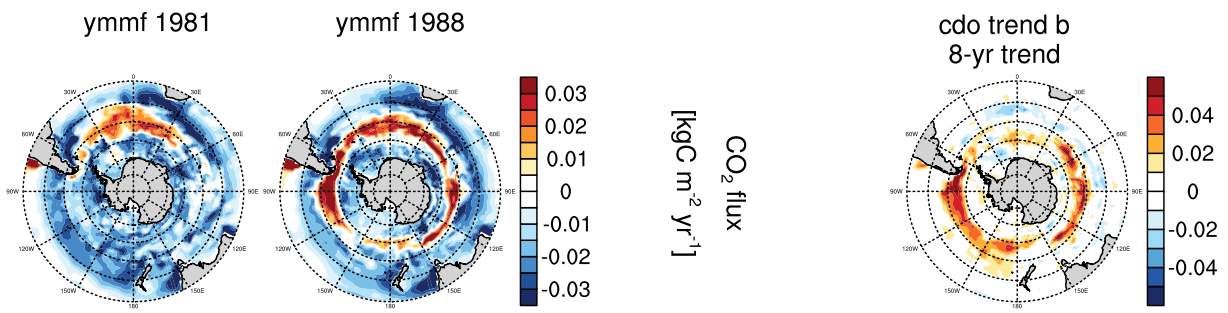
\includegraphics[scale=.55,trim=30cm 0cm 0cm 2.5cm,clip]{co2flux.png}
%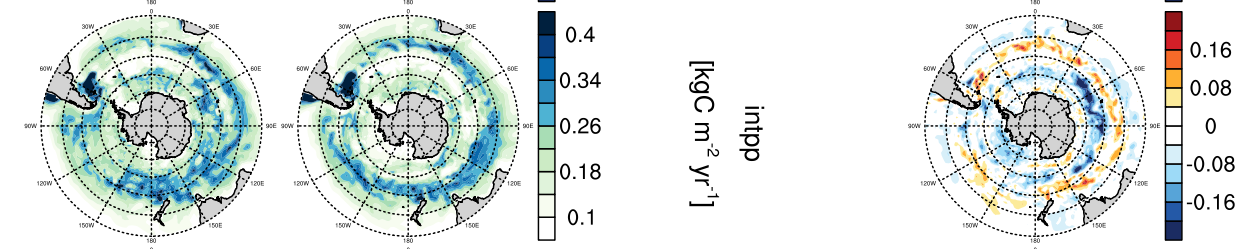
\includegraphics[scale=.55,trim=30cm 0cm 0cm 0.2cm,clip]{intpp.png} % from gfx folder
%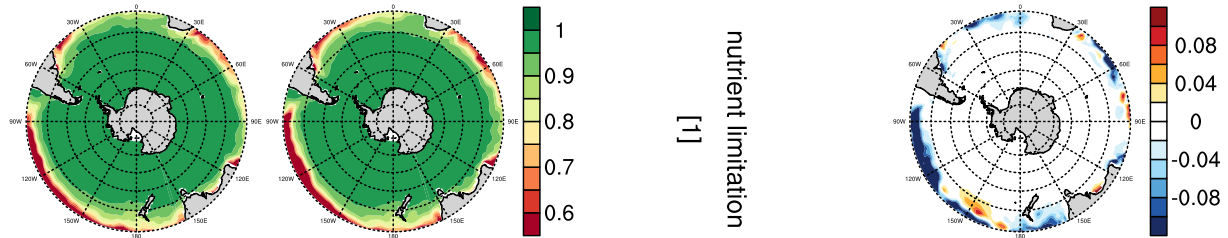
\includegraphics[scale=.75,trim=22cm 0cm 0cm 0cm,clip]{nutrient_limitation.png} % from gfx folder
%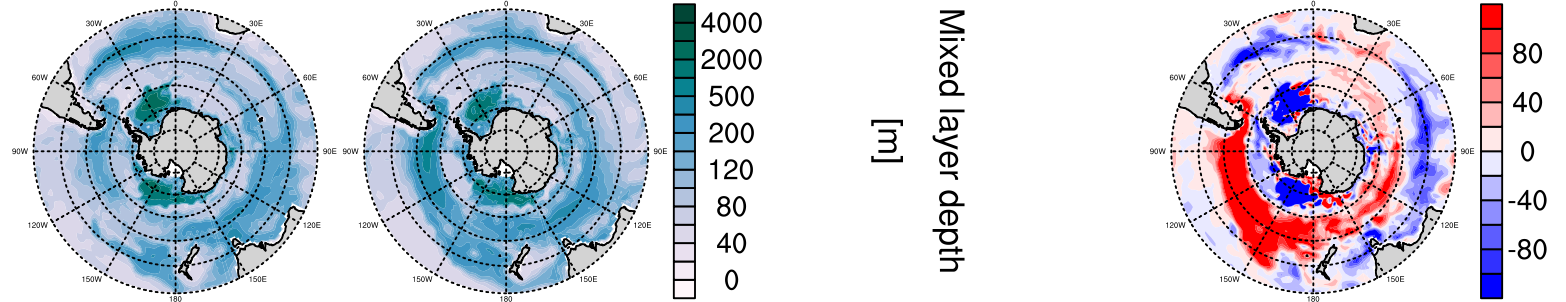
\includegraphics[scale=.55,trim=29cm 0cm 0cm 0cm,clip]{zmld.png} 
%\caption{Trend per per 8 years: CO$_2$flux (top left), vertically integrated primary production trend (top right), nutrient limitation (bottom right) and mixed layer depth (bottom left); hatched areas indicate where trends were below 5\% significance}
%\label{fig:co2flux_intpp}
%\end{figure}

%make it summer trends
\begin{figure}[h]
\includegraphics[scale=1.4,trim=13.25cm 18.7cm 2.5cm 6cm,clip]{\member _positive_trend_8_obgc_overview_summer.pdf} %co2flux
\includegraphics[scale=1.4,trim=13.25cm 15.9cm 2.5cm 9.2cm,clip]{\member _positive_trend_8_obgc_overview_summer.pdf} %intpp
\includegraphics[scale=1.4,trim=13.25cm 13.1cm 2.5cm 12.1cm,clip]{\member _positive_trend_8_obgc_overview_summer.pdf} %nutlimf
\includegraphics[scale=1.4,trim=13.25cm 7.3cm 2.5cm 17.8cm,clip]{\member _positive_trend_8_obgc_overview_summer.pdf} %zmld
\caption{Southern Ocean austral summer trends per per 8 years: CO$_2$flux (top left), vertically integrated primary production (top right), nutrient limitation (bottom right) and mixed layer depth (bottom left); hatched areas indicate where trends were below 5\% significance}
\label{fig:co2flux_intpp}
\end{figure}

However, the mixed layer depth increased in 50-60$^\circ$S (Fig. \ref{fig:co2flux_intpp}). Mixing can bring phytoplankton to deeper levels of the ocean where they are exposed to less light which inhibits plankton growth. Sverdrup \citep{Sverdrup1953} introduced his concept of critical depth based turbulent mixing as a requirement for plankton blooms \citep{Franks2014}. We use his theory not in an overall manner discussing theoretical requirements of the water column for plankton bloom dynamics, but rather the straight-forward effect of mixing plankton to deeper layers. Sverdrup based this theory on turbulent mixing. However, here we use a hydrologically defined mixed layer depth based on a density criterion, which serves as a first approach to wind-induced mixing strength. The direct effect of wind on the water column is described by the vertical diffusivity due to wind. The spatial coexistence/correlation justifies to use of mixed layer depth as an indicator for turbulent wind mixing (Fig. \ref{fig:wind_mixing}).  

To visualize mixing of phytoplankton towards deeper layers, we calculated an average depth of phytoplankton mass based on the mechanics of center of mass. Here, we see an increase in depth at 50-60$^\circ$S indicating deeper mixing and hence less light availability. At 50-60$^\circ$S we see an increase in plankton average depth upto 15m (Fig. \ref{fig:wind_mixing}). This change in depth is accompanied by a decrease of up to ~20\% in solar radiation. As primary production is a highly non-linear process, lower growth rate drastically impacts the plankton bloom.


Deeper winter mixing also effects the plankton bloom as it shortens the available time of a stratified water column required for primary production. The water column in the Southern Ocean is mixed deeply in the winter seasons. In spring, solar radiation restratifies the water column. The more mixing happened in winter and during restratification spring, the longer plankton cannot bloom. So wind-mixing has a two-fold implication on primary production and the carbon sink: It shortens the timeframe for primary production and it deepens a fraction of the standing stock. In 50-60$^\circ$S deeper winter mixing inhibits plankton growth in early spring (Fig. \ref{fig:zmld_intpp_seasonality}). Also throughout the growth season, the mixed depth layer increases about 10m which drags standing stock down to depths with less light.


\begin{figure}[h]
%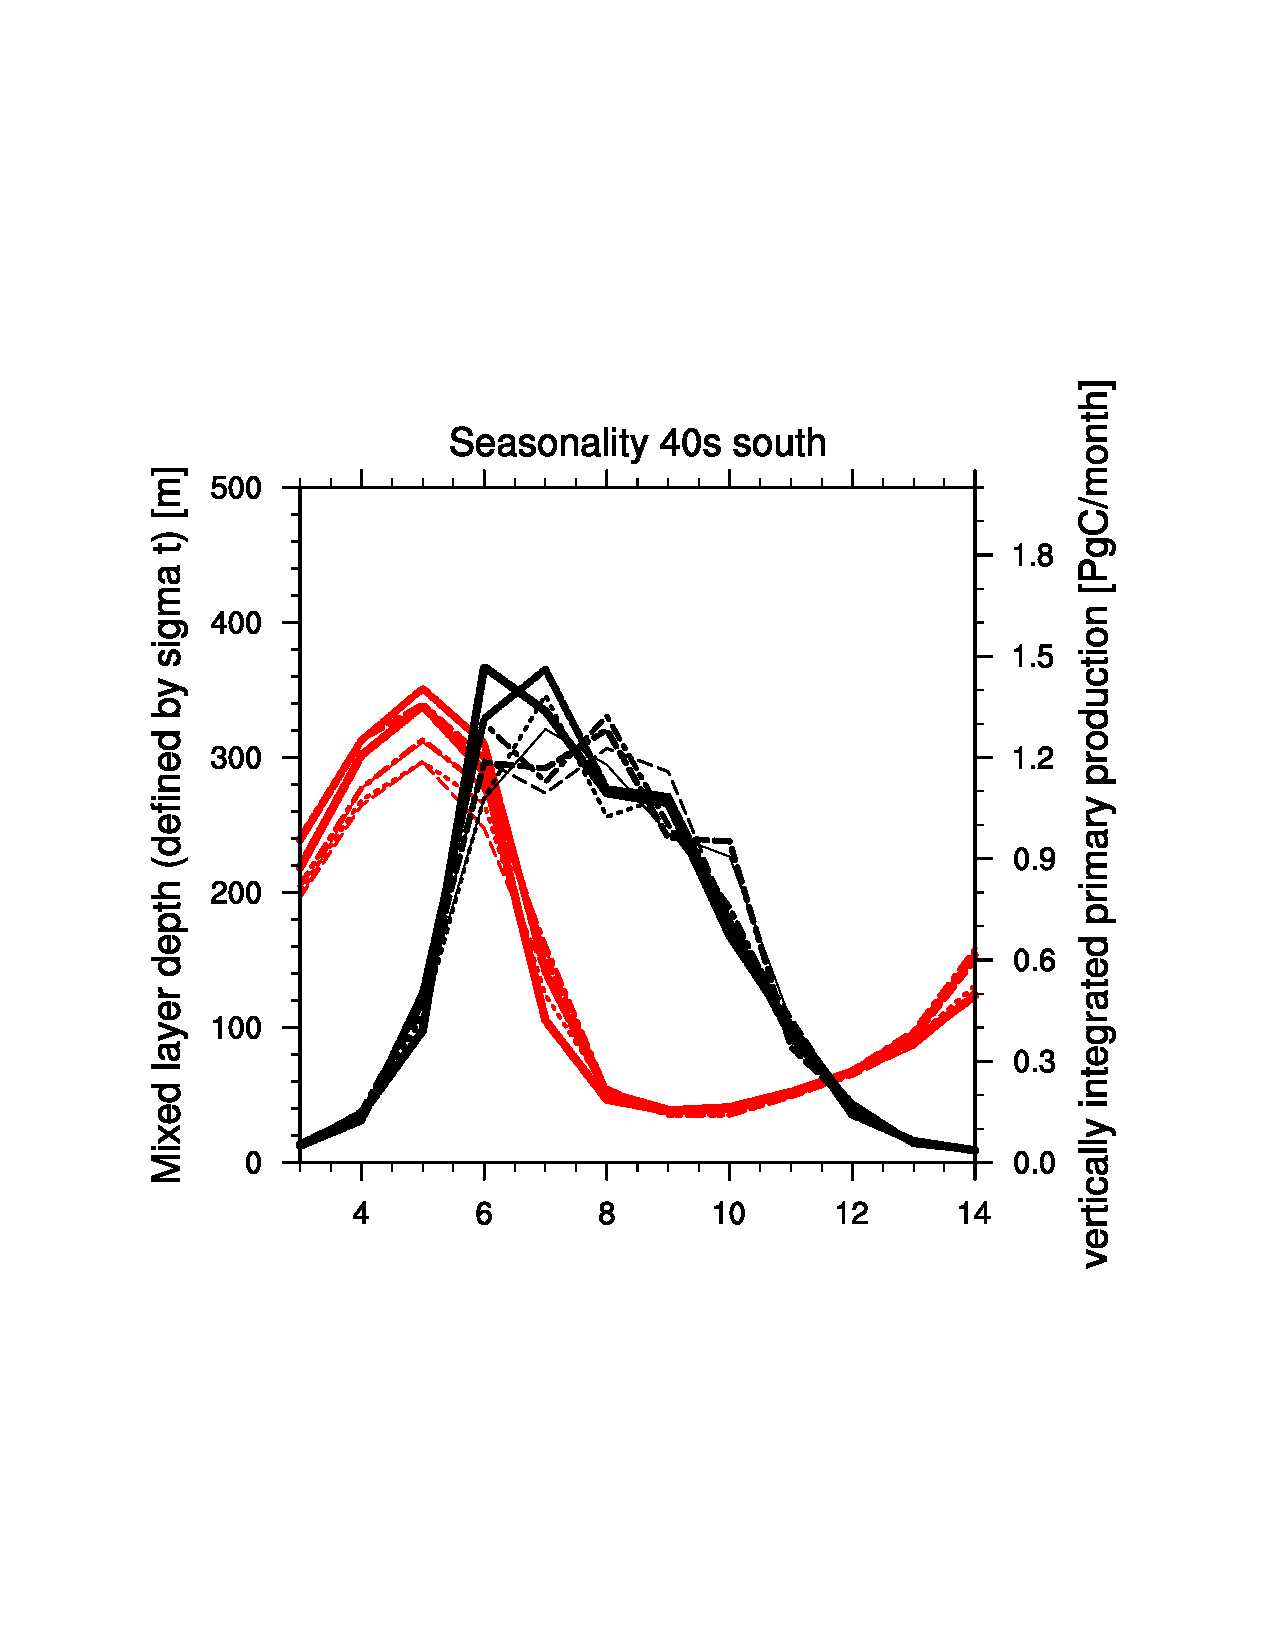
\includegraphics[scale=.4,trim=0cm 6cm 0cm 5cm,clip]{seasonality_intpp_zmld_area40} % from gfx folder
\centering
\includegraphics[page=2,scale=.6,trim=0cm 6cm 0cm 5cm,clip]{\member _positive_trend_8_seasonality_intpp_zmld.pdf} % from gfx folder
%\vspace{-1cm}
\caption{Seasonality of vertically integrated primary production (black) and mixed layer depth (red) at 50-60$^\circ$S over 8 years; thicker lines are later years}
\label{fig:zmld_intpp_seasonality}
\end{figure}

South of 50$^\circ$S experiences an cold SST anomaly due to upwelling? This cooling directly weakens primary production via the Eppley curve. However, this temperature effect also explains why at 40-50$^\circ$S primary production even increases slightly. There is a warm SST anomaly and winds decrease slightly. There is even a slight increase in primary production that may be attributed to a more stratified water column, because additionally to less wind stress, sea-surface temperature experiences a warming trend here.


Previous studies state that intensified wind lead to increased upwelling, which then impacts the surface pCO$_2$ to rise and thereby weaken the carbon uptake. We also see this pattern of intensified winds (Fig. SI \ref{fig:slp_wind}) in a positive trend in SAM (Fig. SI \ref{fig:sam}). Positive trends in SAM deepen the mixed-layer depth and by that lower productivity due to light availability \citep{Sallee2010}.

Increased upwelling brings cold water from the deep ocean. This cools the surface layer. This cold sea-surface temperature anomaly reduces stratification, so wind stress is more effective in mixing the water column.

\begin{figure}
\includegraphics[scale=.85,trim=1.2cm 13.2cm 0cm 7cm,clip]{\member _positive_trend_8_schwerpunkt_mixing_overview.pdf}
\caption{Trends in [m/8yrs] for phytoplankton average depth (left) and average depth of vertical diffusivity due to wind (right); hatched areas indicate where trends were below 5\% significance}
\label{fig:wind_mixing}
\end{figure}


The strong trend in MLD could also be a sign of increasing outgassing due to more mixing. Mixing brings surface water including phytoplankton to deeper layers. This comes in exchange for carbon-rich deep waters.

We were not able to attribute weights on the two follow-up effects on upwelling in the sense of impact on the carbon sink. [Maybe later]



\section{Discussion}
\citep{Lovenduski2005}: how is model different, how are results different
\begin{enumerate}
\item our MLD responds differently than Lovenduski2005 Fig.2 schematic illustration
\item increase in SAM → increase in chlorophyll south of PF/45°S because of iron supply from below (we have phy-decrease)
\item increase in SAM → reduction in chlorophyll north of PF/45°S because of increased ZMLD (we have a slight phy-increase)
\item BUT we dont have iron limitation in SO, so this study can be used as a direct physical effect of stronger winds on primary production excluding nutrient supply changes
\end{enumerate} 

\citep{Hauck2013}: stronger winds, increased upwelling, more iron supply, higher primary production

\citep{wang2012}: 
\begin{enumerate}
\item forced model, 25yr trends, so rather climate change impact than decadal variability
\item some regions: more upwelling, more iron, more primary production 
\item I dont get the clear storyline of the whole paper
\end{enumerate}

Limitations of HAMOCC vs obs/other models:
\begin{enumerate}
\item too early and enhanced Southern Ocean seasonal cycle \citep{Nevison2016}
\item not eddy resolving, has impacts \citep{somestudy}
\item location of polar jets in ECHAM %[I remember this from a group meeting, but didnt check so far]
\item basically no nutrient limitation in SO? - other models and observations disagree
\item other observation studies use sparse for pCO2 or proxy (satelite chl-a)
\item MPIOM performance on circulation patterns and water masses in SO %(Yohei mentioned Anne M. could know this)
\item only one phytoplankton type in HAMOCC? - more variety of plankton species might be able to adapt to depth? or is this too unrealistic for a global model such as HAMOCC?
\item MPI-ESM zmld performance in SO \citep{Sallee2013}
\end{enumerate} 



\section{Summary and conclusions}

MPI-ESM large ensemble simulations produces internal variability of the Southern Ocean carbon sink including decreasing decadal carbon sink trends over the past decades, which were seen in observations. Decreasing carbon sink trends are accompanied by intensified winds as in previous studies \citep{LeQuere2007,Lovenduski2008}. The changes in circulation induce a different response to biology as in previous studies\citep{Lovenduski2005,Hauck2013,wang2012}, which is mainly attributed to differences in nutrient availability. Our results suggest that increasing winds not only enhance upwelling of carbon-rich waters, but also decrease water column stability which inhibits primary production. An overall decrease in primary production decreases the Southern Ocean carbon sink. 


\section*{Acknowledgements}
Thanks to Luis Kornblueh, J{\"u}rgen Kr{\"o}ger, Michael Botzet for making the large ensemble simulations available. The simulations were performed at the Swiss national supercomputing center (CSCS) and the German Climate Computing Center (DKRZ). Primary data and scripts used in the analysis of this study are archived by the Max Planck Institute for Meteorology and can be obtained by contacting publications@mpimet.mpg.de.


\newpage
\baselineskip18pt
%\addbibresource{../Paper/SouthernOceanCarbonSink_new}
\bibliography{../Paper/SouthernOceanCarbonSink_new}

\bibliographystyle{abbrvnat}%unsrtnat}%abbrvnat}%plainnat}

\newpage

\section*{Supplementary information}

\subsection*{Normal distributions of the southern ocean carbon sink}
\begin{figure}[h]
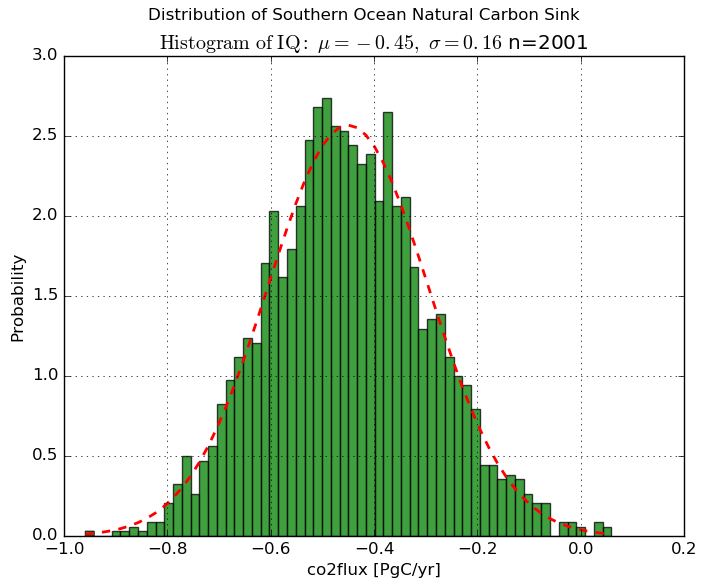
\includegraphics[scale=.4]{SOCS_temporal_gaussian.png} % from gfx folder
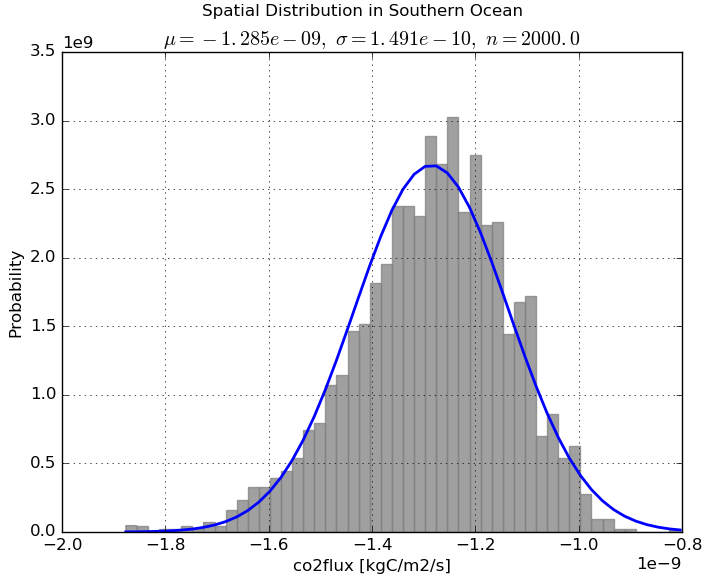
\includegraphics[scale=.4]{SOCS_spatial_gaussian.png} % from gfx folder
\caption{Southern Ocean carbon sink: yearmean fieldsum 35-90S (left) and yearmean in a random grid cell (right)}
\label{fig:SOCS_temporal_gaussian}
\end{figure}

%\begin{figure}[h]
%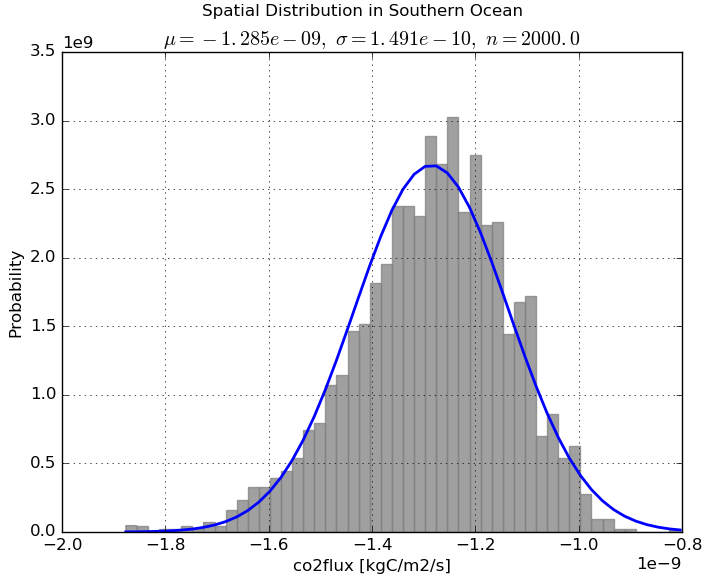
\includegraphics[scale=.5]{SOCS_spatial_gaussian.png} % from gfx folder
%\caption{Southern Ocean carbon sink for a random gridpoint in the Southern Ocean}
%\label{fig:SOCS_spatial_gaussian}
%\end{figure}

%\subsection*{Delta pCO$_2$-separation}
\begin{figure}[h]
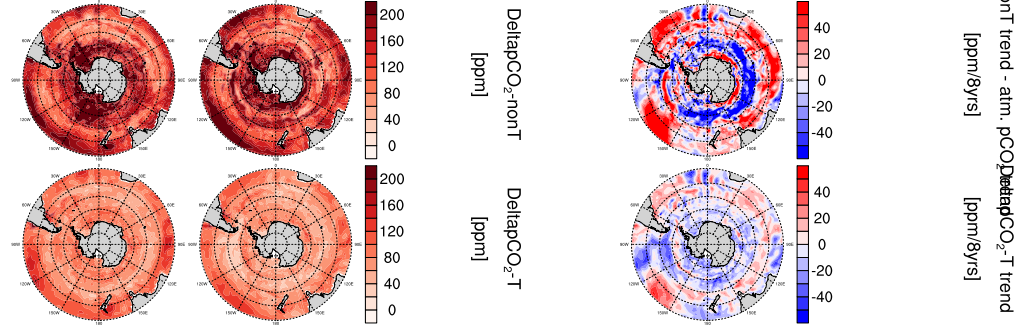
\includegraphics[scale=.6]{dpco2_separation.png} % from gfx folder
\caption{Delta pCO$_2$-separation \citep{Takahashi2002}}
\label{fig:dpco2_separation}
\end{figure}

\newpage
%\subsection*{Misc}
\begin{figure}
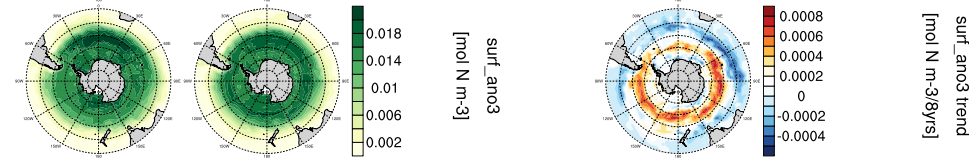
\includegraphics[scale=.6]{nutrients.png} % from gfx folder
\caption{Nutrient}
\label{fig:nutrients}
\end{figure}
\begin{figure}
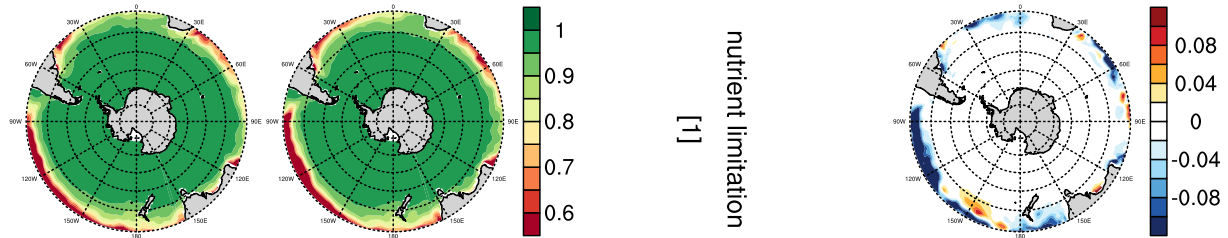
\includegraphics[scale=.45,trim=0cm 0cm 0cm 0cm,clip]{nutrient_limitation.png} % from gfx folder
\caption{Yearmean nutrient limitation for primary production (left) and trend over 8 years (right)}
\label{fig:nutrient_limitation}
\end{figure}
\begin{figure}
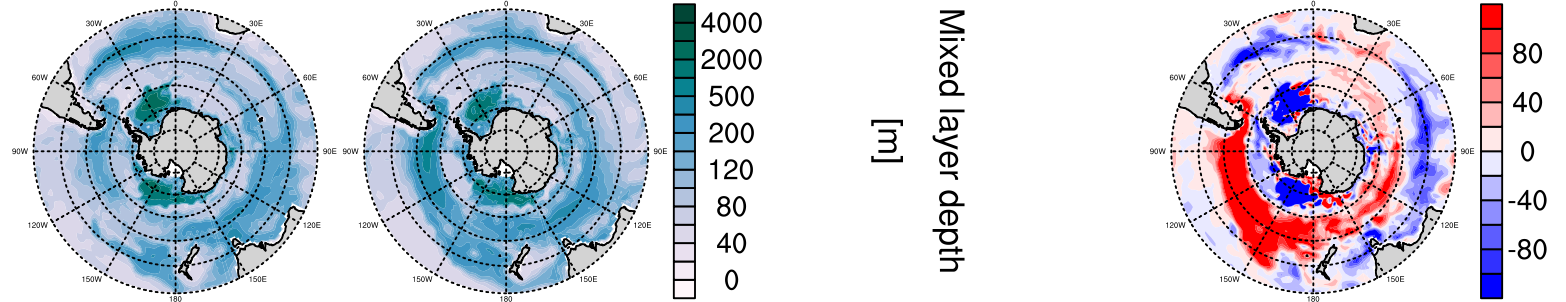
\includegraphics[scale=.35,trim=0cm 0cm 0cm 0cm,clip]{zmld.png} % from gfx folder
\caption{Mixed depth layer in the first and last year of the trend period; trend over 8 years}
\label{fig:zmld}
\end{figure}
\begin{figure}
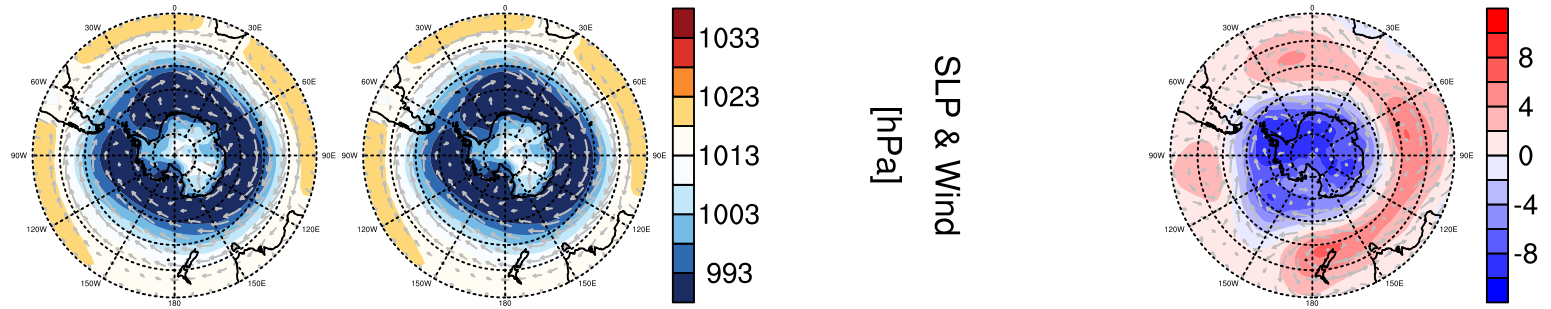
\includegraphics[scale=.35]{slp_wind.png} % from gfx folder
\caption{Sea-level pressure and wind fields in the first and last year of the trend period; trend over 8 years}
\label{fig:slp_wind}
\end{figure}

\clearpage
%\subsection*{Climate Variability}
\begin{figure}[h]
\includegraphics[scale=.2,trim=0cm 0cm 0cm 0cm,clip]{\member _sam_timeseries_son.png} % from gfx folder
\caption{SAM timeseries for September, October and November}
%\label{fig:sam}
%\end{figure}
%\begin{figure}[h]
\includegraphics[scale=.2,trim=0cm 0cm 0cm 0cm,clip]{\member _nino34_timeseries.png} % from gfx folder
%\caption{elnino 3.4 timeseries}
%\label{fig:nino34}
%\end{figure}
%\begin{figure}[h]
\includegraphics[scale=.2,trim=0cm 0cm 0cm 0cm,clip]{\member _pdo_timeseries.png} % from gfx folder
%\caption{PDO timeseries}
%\label{fig:pdo}
\caption{Timeseries of SAM, El Nino and PDO}
\label{fig:CVDP}
\end{figure}

\clearpage

\includepdf{/home/mpim/m300524/MSc_Thesis/gfx/\member  _positive_trend_8_obgc_overview_summer.pdf}
\includepdf{/home/mpim/m300524/MSc_Thesis/gfx/\member  _positive_trend_8_obgc_overview_winter.pdf}
\includepdf{/home/mpim/m300524/MSc_Thesis/gfx/\member  _positive_trend_8_pco2_overview.pdf}


\clearpage


%\subsection*{Landschuetzer plots}
\begin{figure}
\centering
\includegraphics[scale=1.1,trim=5cm 5cm 6cm 5.5cm,clip]{\member _positive_trend_8_Landschuetzer_overview.pdf}
\caption{\citep{landschuetzer2015} Fig. 2}
\label{fig:landschuetzer}
\end{figure}
\begin{figure}
\centering
\includegraphics[scale=1.1,trim=5cm 5cm 6cm 5.5cm,clip]{\member _positive_trend_8_Landschuetzer_summer_overview.pdf}
\caption{\citep{landschuetzer2015} SI sommer}
\label{fig:landschuetzer_summer}
\end{figure}
\begin{figure}
\centering
\includegraphics[scale=1.1,trim=5cm 5cm 6cm 5.5cm,clip]{\member _positive_trend_8_Landschuetzer_winter_overview.pdf}
\caption{\citep{landschuetzer2015} SI winter}
\label{fig:landschuetzer_winter}
\end{figure}

\clearpage

\subsection*{Selection criteria for decadal trend members}
\begin{enumerate}
\item positive CO2flux trend: value PgC/yr
\item monotony Mann-Kendall
\item significance student t-Test
\end{enumerate}

\end{document}




















